\documentclass{article}\usepackage[]{graphicx}\usepackage[]{color}
%% maxwidth is the original width if it is less than linewidth
%% otherwise use linewidth (to make sure the graphics do not exceed the margin)
\makeatletter
\def\maxwidth{ %
  \ifdim\Gin@nat@width>\linewidth
    \linewidth
  \else
    \Gin@nat@width
  \fi
}
\makeatother

\definecolor{fgcolor}{rgb}{0.345, 0.345, 0.345}
\newcommand{\hlnum}[1]{\textcolor[rgb]{0.686,0.059,0.569}{#1}}%
\newcommand{\hlstr}[1]{\textcolor[rgb]{0.192,0.494,0.8}{#1}}%
\newcommand{\hlcom}[1]{\textcolor[rgb]{0.678,0.584,0.686}{\textit{#1}}}%
\newcommand{\hlopt}[1]{\textcolor[rgb]{0,0,0}{#1}}%
\newcommand{\hlstd}[1]{\textcolor[rgb]{0.345,0.345,0.345}{#1}}%
\newcommand{\hlkwa}[1]{\textcolor[rgb]{0.161,0.373,0.58}{\textbf{#1}}}%
\newcommand{\hlkwb}[1]{\textcolor[rgb]{0.69,0.353,0.396}{#1}}%
\newcommand{\hlkwc}[1]{\textcolor[rgb]{0.333,0.667,0.333}{#1}}%
\newcommand{\hlkwd}[1]{\textcolor[rgb]{0.737,0.353,0.396}{\textbf{#1}}}%

\usepackage{framed}
\makeatletter
\newenvironment{kframe}{%
 \def\at@end@of@kframe{}%
 \ifinner\ifhmode%
  \def\at@end@of@kframe{\end{minipage}}%
  \begin{minipage}{\columnwidth}%
 \fi\fi%
 \def\FrameCommand##1{\hskip\@totalleftmargin \hskip-\fboxsep
 \colorbox{shadecolor}{##1}\hskip-\fboxsep
     % There is no \\@totalrightmargin, so:
     \hskip-\linewidth \hskip-\@totalleftmargin \hskip\columnwidth}%
 \MakeFramed {\advance\hsize-\width
   \@totalleftmargin\z@ \linewidth\hsize
   \@setminipage}}%
 {\par\unskip\endMakeFramed%
 \at@end@of@kframe}
\makeatother

\definecolor{shadecolor}{rgb}{.97, .97, .97}
\definecolor{messagecolor}{rgb}{0, 0, 0}
\definecolor{warningcolor}{rgb}{1, 0, 1}
\definecolor{errorcolor}{rgb}{1, 0, 0}
\newenvironment{knitrout}{}{} % an empty environment to be redefined in TeX

\usepackage{alltt}

\usepackage{amsmath}
\usepackage{amsthm}
\usepackage{amsfonts}
\usepackage{hyperref}


\title{Meeting 3}
\author{Anh Le}
\IfFileExists{upquote.sty}{\usepackage{upquote}}{}
\begin{document}

\maketitle

\section{Readings}

Read Sec. 1.4, Functions, operators, and loops.

This is where you start thinking like a programmer. Up until now, we have only learned names of commands, what are their options, etc. Basically, instead of point-and-click in Excel, we now type into RStudio.

On the other hand, functions and loops are the real ``logic'' of programming and will make you very powerful. We don't point-and-click anymore, but write guidances for the computer to point-and-click for us.

Consider the following function that is trivial to write but very useful in real (grad) life. Suppose your advisor told you to calculate the summary statistics of ALL the variable in the dataset.

\begin{knitrout}
\definecolor{shadecolor}{rgb}{0.969, 0.969, 0.969}\color{fgcolor}\begin{kframe}
\begin{alltt}
\hlstd{data} \hlkwb{<-} \hlkwd{data.frame}\hlstd{(}\hlkwc{var1}\hlstd{=}\hlkwd{rnorm}\hlstd{(}\hlnum{10}\hlstd{,} \hlkwc{mean}\hlstd{=}\hlnum{0}\hlstd{,} \hlkwc{sd}\hlstd{=}\hlnum{1}\hlstd{),}
                   \hlkwc{var2}\hlstd{=}\hlkwd{rnorm}\hlstd{(}\hlnum{10}\hlstd{,} \hlkwc{mean}\hlstd{=}\hlnum{2}\hlstd{,} \hlkwc{sd}\hlstd{=}\hlnum{5}\hlstd{),}
                   \hlkwc{var3}\hlstd{=}\hlkwd{runif}\hlstd{(}\hlnum{10}\hlstd{,} \hlkwc{min}\hlstd{=}\hlnum{1}\hlstd{,} \hlkwc{max}\hlstd{=}\hlnum{6}\hlstd{))}
\hlstd{data}
\end{alltt}
\begin{verbatim}
##        var1    var2  var3
## 1  -0.17069  2.5044 5.273
## 2   0.38687 -8.3671 2.219
## 3   0.72805 12.4770 5.809
## 4  -0.72370 -0.7633 2.312
## 5  -0.40455  2.8970 2.024
## 6  -0.09673  1.7595 4.119
## 7   0.71740 -1.6797 5.212
## 8   1.17321 -2.7695 1.522
## 9   0.04649  1.2906 5.887
## 10 -1.12565 11.7990 2.329
\end{verbatim}
\end{kframe}
\end{knitrout}

Now, if we know some R but still in the ``point-and-click'' stage, we will write something like this:

\begin{knitrout}
\definecolor{shadecolor}{rgb}{0.969, 0.969, 0.969}\color{fgcolor}\begin{kframe}
\begin{alltt}
\hlkwd{mean}\hlstd{(data}\hlopt{$}\hlstd{var1)}
\end{alltt}
\begin{verbatim}
## [1] 0.05307
\end{verbatim}
\begin{alltt}
\hlkwd{sd}\hlstd{(data}\hlopt{$}\hlstd{var1)}
\end{alltt}
\begin{verbatim}
## [1] 0.7101
\end{verbatim}
\begin{alltt}
\hlkwd{mean}\hlstd{(data}\hlopt{$}\hlstd{var2)}
\end{alltt}
\begin{verbatim}
## [1] 1.915
\end{verbatim}
\begin{alltt}
\hlkwd{sd}\hlstd{(data}\hlopt{$}\hlstd{var2)}
\end{alltt}
\begin{verbatim}
## [1] 6.313
\end{verbatim}
\begin{alltt}
\hlkwd{mean}\hlstd{(data}\hlopt{$}\hlstd{var3)}
\end{alltt}
\begin{verbatim}
## [1] 3.67
\end{verbatim}
\begin{alltt}
\hlkwd{sd}\hlstd{(data}\hlopt{$}\hlstd{var3)}
\end{alltt}
\begin{verbatim}
## [1] 1.755
\end{verbatim}
\end{kframe}
\end{knitrout}

So instead of ``point-and-click'' 6 times in Excel, we wrote 6 lines in R. Still do-able.

But God forbid, what if the dataset has 100 variables? What if we need more summary statistic than just \verb`mean` and \verb`sd`? Functions to the rescue.

\begin{knitrout}
\definecolor{shadecolor}{rgb}{0.969, 0.969, 0.969}\color{fgcolor}\begin{kframe}
\begin{alltt}
\hlstd{my_summary_statistic_function} \hlkwb{<-} \hlkwa{function}\hlstd{(}\hlkwc{data_vector}\hlstd{) \{}
  \hlstd{mean_of_data} \hlkwb{<-} \hlkwd{mean}\hlstd{(data_vector,} \hlkwc{na.rm}\hlstd{=}\hlnum{TRUE}\hlstd{)}
  \hlstd{median_of_data} \hlkwb{<-} \hlkwd{median}\hlstd{(data_vector,} \hlkwc{na.rm}\hlstd{=}\hlnum{TRUE}\hlstd{)}
  \hlstd{sd_of_data} \hlkwb{<-} \hlkwd{sd}\hlstd{(data_vector,} \hlkwc{na.rm}\hlstd{=}\hlnum{TRUE}\hlstd{)}

  \hlstd{result} \hlkwb{<-} \hlkwd{c}\hlstd{(mean_of_data, median_of_data, sd_of_data)}
  \hlkwd{names}\hlstd{(result)} \hlkwb{<-} \hlkwd{c}\hlstd{(}\hlstr{"mean"}\hlstd{,} \hlstr{"median"}\hlstd{,} \hlstr{"standard deviation"}\hlstd{)}

  \hlkwd{return}\hlstd{(result)}
\hlstd{\}}

\hlkwd{my_summary_statistic_function}\hlstd{(data}\hlopt{$}\hlstd{var1)}
\end{alltt}
\begin{verbatim}
##               mean             median standard deviation 
##            0.05307           -0.02512            0.71007
\end{verbatim}
\begin{alltt}
\hlkwd{my_summary_statistic_function}\hlstd{(data}\hlopt{$}\hlstd{var2)}
\end{alltt}
\begin{verbatim}
##               mean             median standard deviation 
##              1.915              1.525              6.313
\end{verbatim}
\begin{alltt}
\hlkwd{my_summary_statistic_function}\hlstd{(data}\hlopt{$}\hlstd{var3)}
\end{alltt}
\begin{verbatim}
##               mean             median standard deviation 
##              3.670              3.224              1.755
\end{verbatim}
\end{kframe}
\end{knitrout}

We have just created a \textbf{re-usable} function that can take in any vector of data and spits out our desirable statistic. If the advisor at some point wants us to add a statistic, we only have to add that statistic to our function.

And lastly, instead of using our \verb`my_summary_statistic_function` on each column by hand, we can also tell R to do it as follows:

\begin{knitrout}
\definecolor{shadecolor}{rgb}{0.969, 0.969, 0.969}\color{fgcolor}\begin{kframe}
\begin{alltt}
\hlkwd{apply}\hlstd{(data,} \hlkwc{MARGIN}\hlstd{=}\hlnum{2}\hlstd{,} \hlkwc{FUN}\hlstd{=my_summary_statistic_function)}
\end{alltt}
\begin{verbatim}
##                        var1  var2  var3
## mean                0.05307 1.915 3.670
## median             -0.02512 1.525 3.224
## standard deviation  0.71007 6.313 1.755
\end{verbatim}
\begin{alltt}
\hlcom{# Equivalently, we can use loop}
\hlkwa{for} \hlstd{(i} \hlkwa{in} \hlnum{1}\hlopt{:}\hlkwd{ncol}\hlstd{(data)) \{}
  \hlkwd{print}\hlstd{(}\hlkwd{my_summary_statistic_function}\hlstd{(data[ , i]))}
\hlstd{\}}
\end{alltt}
\begin{verbatim}
##               mean             median standard deviation 
##            0.05307           -0.02512            0.71007 
##               mean             median standard deviation 
##              1.915              1.525              6.313 
##               mean             median standard deviation 
##              3.670              3.224              1.755
\end{verbatim}
\end{kframe}
\end{knitrout}

\section{In-class Exercises}

\begin{enumerate}
\item See \href{http://polsci630.herokuapp.com/meetings}{our website}.
\item Trivial: \verb`print("Hello World!")` 100 times.
\item Less trivial: \verb`print("Hello friend #1!")`, \verb`print("Hello friend #2!")`, etc. 100 times
\item Decidedly not trivial: Prove the Central limit theorem with simulation.

First, the Central Limit Theorem (CLT)--the most important theorem in statistics--states that the mean of a random variable is normally distributed, \textbf{regardless of the distribution of the random variable itself}

For example, let's say that $X$ is uniformly distributed between 0 and 1

\begin{knitrout}
\definecolor{shadecolor}{rgb}{0.969, 0.969, 0.969}\color{fgcolor}\begin{kframe}
\begin{alltt}
\hlstd{X} \hlkwb{<-} \hlkwd{runif}\hlstd{(}\hlnum{10000}\hlstd{,} \hlkwc{min}\hlstd{=}\hlnum{0}\hlstd{,} \hlkwc{max}\hlstd{=}\hlnum{1}\hlstd{)}
\hlkwd{mean}\hlstd{(X)}
\end{alltt}
\begin{verbatim}
## [1] 0.4951
\end{verbatim}
\begin{alltt}
\hlkwd{plot}\hlstd{(}\hlkwd{density}\hlstd{(X))}
\end{alltt}
\end{kframe}
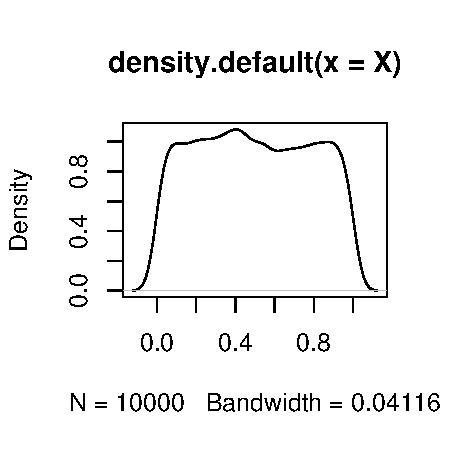
\includegraphics[width=\maxwidth]{figure/unnamed-chunk-5} 

\end{knitrout}

Clearly, the distribution of X is not normal. If we generate X many times (says, $n$ times), and each time calculate its mean, then we will get a vector containing $n$ means. The CLT states that these $n$ means will be normally distributed. (It's amazing! Where does the normal come from??)

Prove it using for loop. Hint: \verb`for (i in 1:n) { do stuff in here }`

\end{enumerate}

\end{document}
